\chapter{Smoothing}\label{ch:smoothing}

Before extracting the features I applied a symmetric smoothing kernel to the image projections. 

Shown in the following are the results with different kernel sizes:

\begin{figure}[ht]
    \centering
    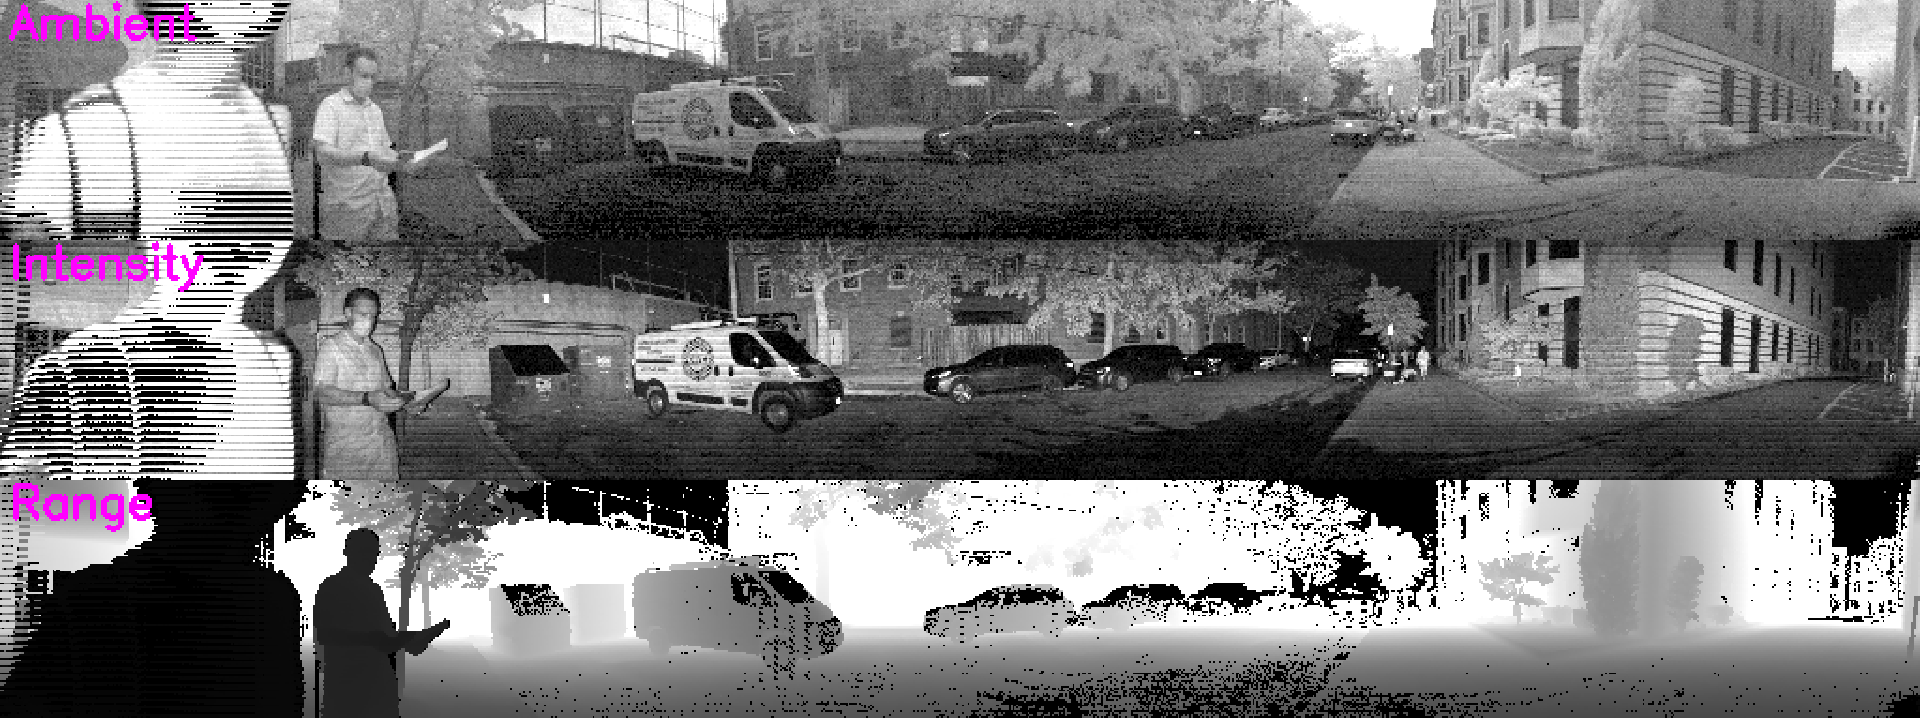
\includegraphics[scale = 0.19]{images/smoothing/no_blur.png}
    \caption{No blur}
\end{figure}

\begin{figure}[ht]
    \centering
    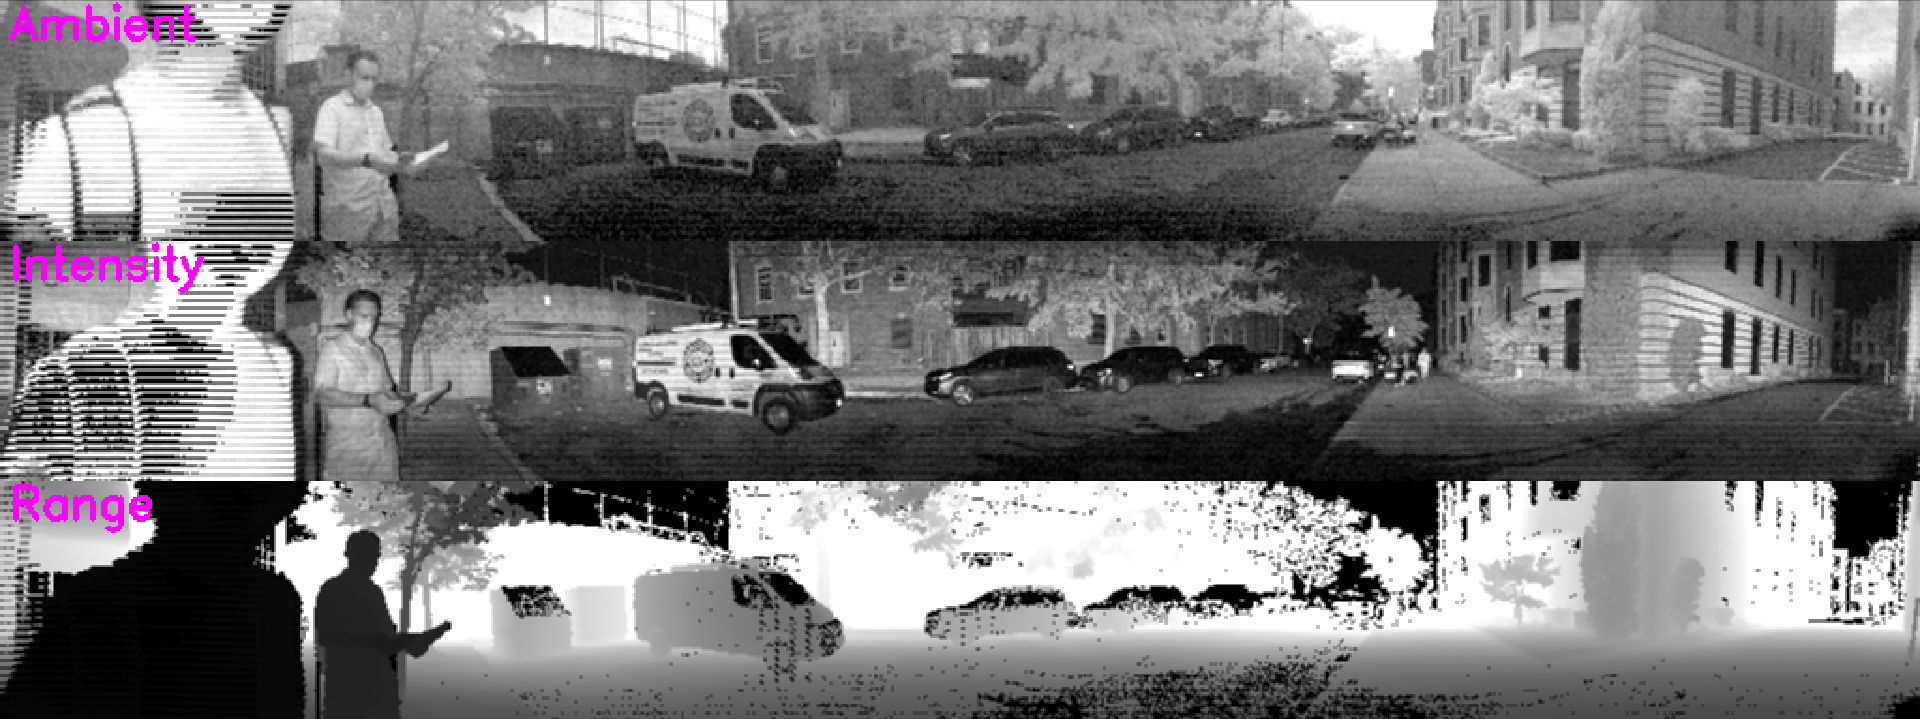
\includegraphics[scale = 0.19]{images/smoothing/2blur.png}
    \caption{Kernel Size of 2 Pixels}
\end{figure}

\clearpage

\begin{figure}[ht]
    \centering
    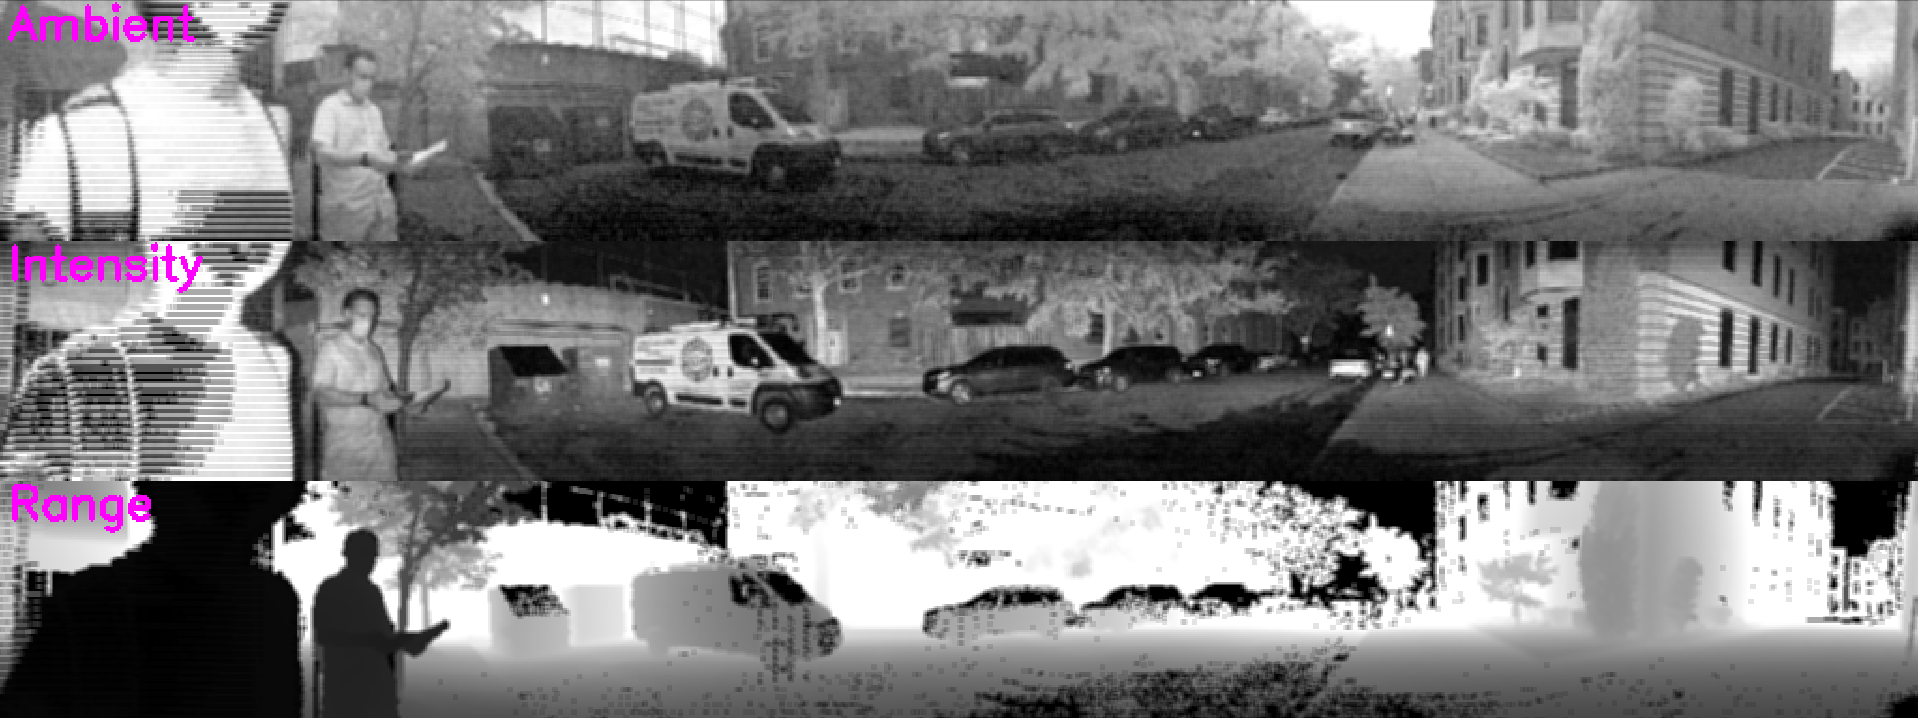
\includegraphics[scale = 0.19]{images/smoothing/3blur.png}
    \caption{Kernel Size of 3 Pixels}
\end{figure}

\begin{figure}[ht]
    \centering
    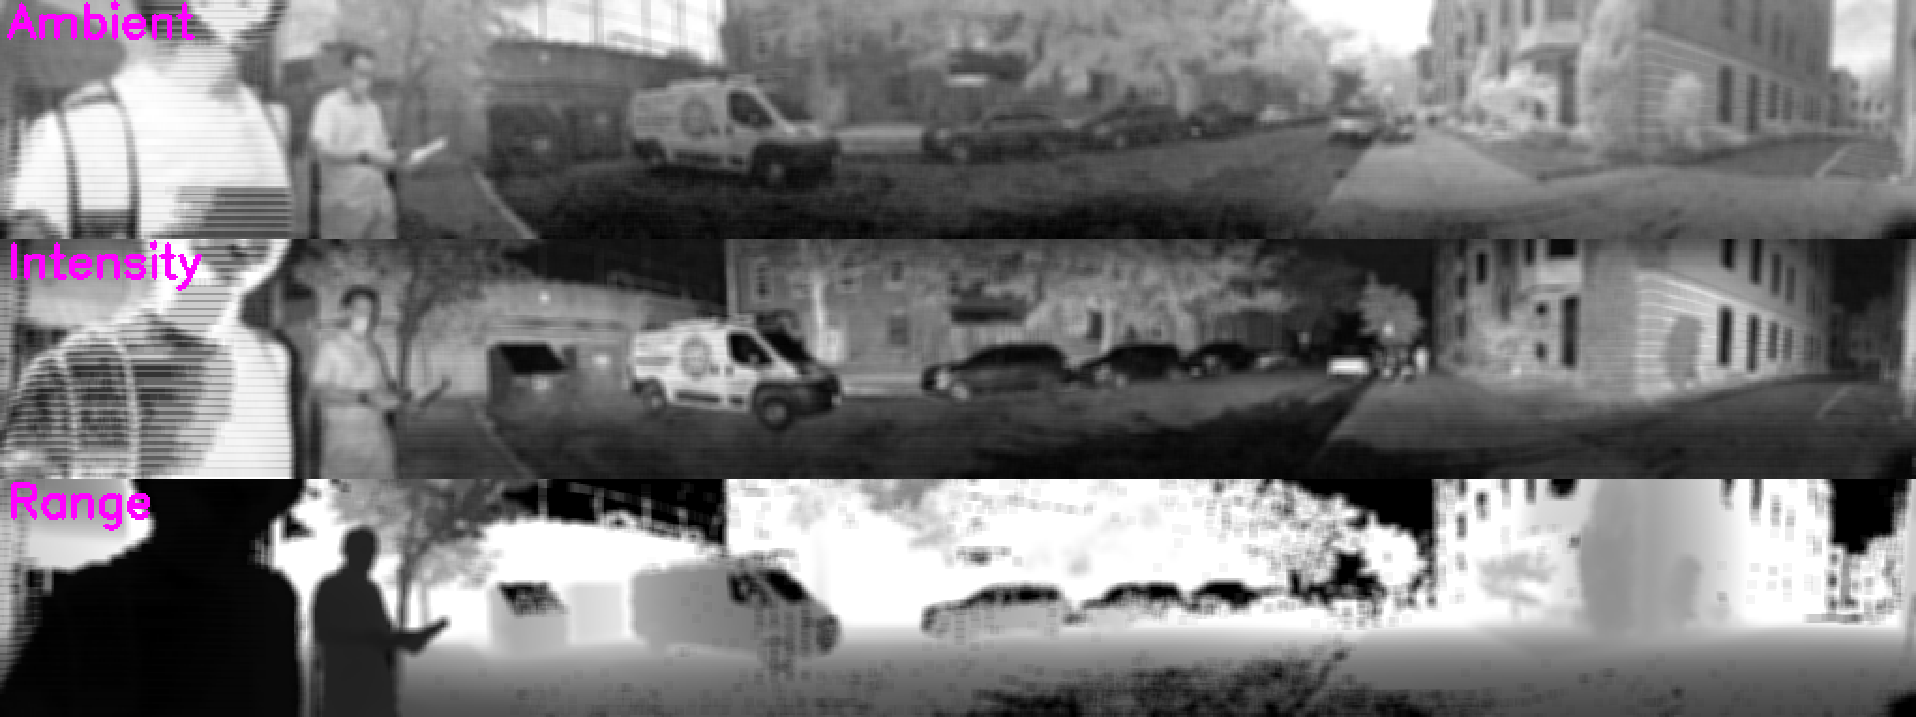
\includegraphics[scale = 0.19]{images/smoothing/5blur.png}
    \caption{Kernel Size of 5 Pixels}
\end{figure}

When calibrating my pipeline the best results seemed to emerge for a kernel with the size of 2 Pixels however I encourage anyone applying these methods to find the best performing settings for their own work.